\subsection{Blockchain}
\label{sec:sota_blockchain}

    {\footnotesize Quellen: \cite{Dorri2016}\cite{Conoscenti2016}\cite{Greenspan2015}\cite{ISO307}\cite{Kshetri2017}\cite{Nakamoto2008}\cite{Underwood2016}\cite{Vukolic2016}\cite{Vukolic2017}\cite{Wuest2017}\cite{Zheng2017}}
    
    Eine Blockchain ist in ihrer Essenz eine immer länger werdende, unveränderbare, öffentliche Kette von Transaktionen, die dezentral gespeichert wird (s. \fref{fig:bc_highlvl}). 
    \smallskip
    \begin{figure}[H]
    	\centering
    	\includegraphics[width=\textwidth]{graphics/bc_highlvl.png}
    	\caption[Abstrakte Darstellung einer Blockchain]{Abstrakte Darstellung einer Blockchain. Jeder neu hinzugefügte Block (hier immer rechts angehängt) enthält eine Referenz auf den Vorigen mittels dessen Hashwert.}
    	\label{fig:bc_highlvl}
    \end{figure}
    \todo[color=yellow]{Transaktionen in m umbenennen (zu Hause}
    \noindent Erstmals 2008 von Satoshi Nakamoto, ursprünglich als Peer-to-Peer Electronic Cash System ,,Bitcoin``
    \!\footnote{Heute werden Bitcoin, Ether, Ripple und andere als digitale Zahlungsmittel als sogennante Kryptowährung bezeichnet} 
    erfunden, erregte die Technologie aufgrund ihrer Eigenschaften wie ihres dezentralen, anonymen Konzepts schnell Aufmerksamkeit. 
    Bitcoin ist die erste populäre digitale Währung, die ohne zentrale Autorität wie beispielsweise einer \gls{ttp} das in \fref{sec:sota_doublespend} vorgestellte Double-Spending Problem lösen sollte\cite{Nakamoto2008}. 
    Übertragen auf Bitcoin bedeutet es, dass ein Empfänger einer Transaktion sichergehen können muss, dass der vorige Besitzer den Bitcoin oder den Bruchteil dessen vorher nicht schon einmal erfolgreicht an einen anderen Empfänger gesendet hat.
    Dies wird mittels kryptographischem Beweis, welcher im folgenden Abschnitt genauer betrachtet wird, anstatt des laut \citeauthor{Nakamoto2008} vorstellten mangelhaften Modells der \gls{ttp}, welche stets einen Single Point of Failure
    \!\footnote{Ein Single Point of Failure stellt beipsielsweise eine Bank im Zahlungsverkehr dar.
    Fällt die Bank beispsielsweise aus irgendeinem Grund aus oder wird kompromittiert, haben deren Kunden keine Möglichkeit mehr sicher Überweisungen von und zu ihren Konten zu tätigen.}
    darstellt, gelöst. 
    Das Konzept ermöglicht es somit zwei Entitäten, auch wenn sie sich gegenseitig nicht vertrauen, eine sichere (im Sinne der Vertraulichkeit) direkte Transaktion miteinander durchzuführen.
    
    \subsubsection{Einführung in das Konzept}
    \label{sec:sota_blockchain_introduction}
    
    Grundlegend ist die Blockchain eine verteilte Datenstruktur, die zwischen den Mitgliedern eines Netzwerkes repliziert und geteilt wird\cite{Christidis2016}.
    Die Blockchain beinhaltet das maßgebliche ,,Hauptbuch'` von vergangenen Transaktionen, ein Log, dessen Einträge mit Zeitstempeln jeweils zu unterschiedlichen Blöcken zusammengefasst werden. 
    
    Der aktuelle Zustand ergibt sich durch das Zurückverfolgen der einzelnen Transaktionen in der Blockchain. 
    Es wird also kein aktueller Stand, welcher Teilnehmer des Netzwerks was besitzt, gespeichert. 
    
    Jeder Knoten des Netzwerkes (genannt ,,Miner'`) hat stets eine eigene Kopie der Blockchain und fügt validierte, gegenseitig abgestimmte Transaktionen zwischen Teilnehmern hinzu.
    Später zu Blöcken gebündelt.
    
    Nutzer nehmen an dem Netzwerk über einen Knoten teil, wobei der Knoten auch für mehrere Nutzer einen Zugang bieten kann. 
    
    %% Transaktionen
    Getätigte Transaktionen sollen nicht mehr rückgängig gemacht werden können.
    Erreicht wird dies, indem die Rückrechnung des Beweises rechnerisch zu aufwändig sein soll\cite{Nakamoto2008}.
    Somit wird der Verkäufer vor Täuschung geschützt und Treuhandmechanismen können einfach implementiert werden\cite{Nakamoto2008}.  
    
    Es müssen also alle Teilnehmer in einem Bitcoin-Netzwerk alle Transaktionen innerhalb des Netzwerkes kennen.
    Ebenso müssen alle Transaktionen für alle Teilnehmer einsehbar sein, also veröffentlicht werden.
    Weiterhin benötigt das System eine einzige Historie, in welcher alle vergangenen Transaktionen in der Reihenfolge ihres Auftretens stehen.
    Zuletzt benötigt der Empfänger des Coins einen Beweis, dass sich die Mehrheit der Konten zur Zeit der Transaktion einig waren, dass die aktuelle die erste entgegengenommene Transaktion des Coins ist. 
    \cite{Nakamoto2008}
    \todo[color=cyan]{timestamps?}
    
    \subsubsection{Transaktionen}
    \label{sec:sota_blockchain_trx}
	    Zunächst wurde mit digitalen Coins gehandelt, welche einer in Form einer Kette digitaler Signaturen modelliert wurden\cite{Nakamoto2008}.
	    In anderen Anwendungsbereichen außerhalb des Bereiches der Kryptowährungen wird von generalisierten Assets gesprochen.\todo[color=yellow]{richtig?}
	    \begin{figure}[H]
	    	\centering
	    	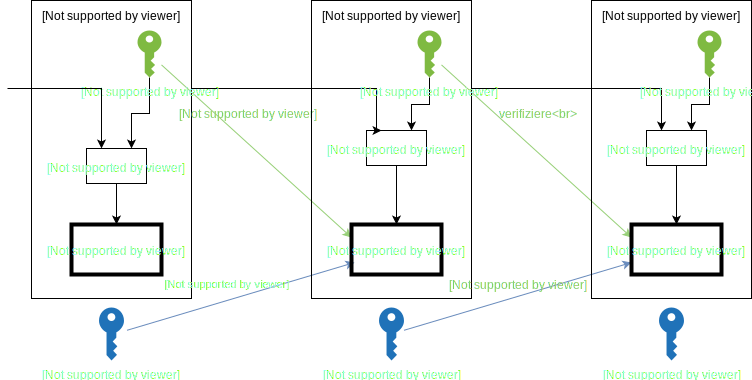
\includegraphics[width=0.9\textwidth]{graphics/transaction.png}
	    	\caption{Kette digitaler Signaturen}
	    	\label{fig:txio}
	    \end{figure}
    
	    Wie in \fref{fig:txio} dargestellt, werden Assets von einem Versender zu einem Empfänger transferiert, in dem der Sender einen Hash der vorigen Transaktion und den öffentlichen Schlüssel des Empfängers mit seinem eigenen privaten Schlüssel digital signiert und diese Hash dann am Ende des Assets anfügt.
	    Transaktionen können zudem mehrere Ein- und Ausgaben haben\cite{Nakamoto2008}.
	    Der Empfänger, sowie alle Teilnehmer des Netzwerkes können den Besitz des Assets über die Kette der digitalen Signaturen zurückverfolgen\cite{Nakamoto2008}.
	    
	    Every signed transaction is broadcasted by a user’s node to its one-hop peers\cite{Christidis2016}
	    
	    The neighboring peers make sure this incoming transaction is valid before relaying it any further; invalid transactions are discarded. Eventually this transaction is spread across the entire network\cite{Christidis2016}
	    
	    The transactions that have been collected and validated by the network using the process above during an agreed-upon time interval, are ordered and packaged into a timestamped candidate block. This is a process called mining. The mining node broadcasts this block back to the network. (The choice of the mining node and the contents of the block depend on the consensus mechanism that the network employs. Refer to Section II-B for more information.)
	    The nodes verify that the suggested block (a) contains valid transactions, and (b) references via hash the correct previous block on their chain. If that is the case, they add the block to their chain, and apply the transactions it contains to update their world view. If that is not the case, the proposed block is discarded. This marks the end of a round.\cite{Christidis2016}
	    
    
    \begin{figure}[H]
        \missingfigure[figheight=4cm]{Bild mit Transaktion}
    \end{figure}
    
    \subsubsection{Smart Contracts}
    
    \subsubsection{Typen}
        Private, Public - Permissioned, Permissionless
        
        Mit einer Blockchain können auch je nach Anwendungsszenario, außer Kryptowährungen, andere (digital repräsentierte) Waren oder Assets wie Güter im Supply Chain Management\cite{Underwood2016}, Identitäten zur Zugangskontrolle\cite{Kshetri2017} oder Proof of Ownership digitaler Rechte\cite{Wuest2017} gespeichert und gehandelt werden. 
        Unterschiedliche Anwendungen haben auch verschiedene Anforderungen an die Blockchain selbst. 
        Zur Zeit haben sich unterschiedliche Typen einer Blockchain herauskristallisiert, wo.
        
        
        {\sloppy\url{https://blockchainhub.net/blockchains-and-distributed-ledger-technologies-in-general/}}
        \begin{itemize}[noitemsep]
            \item in private/\-permissioned ist \gls{pow} und \gls{pos} nicht nötig
        \end{itemize}
    
    \subsubsection{Sicherheit}
    \label{sec:sota_blockchain_security}
        Das System ist so lange sicher, wie ,,ehrliche'` Knoten gemeinsam mehr Rechenleistung als eventuell zusammenarbeitende Angreifer haben\cite{Nakamoto2008}
        Byzantine Fault Tolerance
        Consensus Algorithms
        \begin{itemize}
            \item Users interact with the blockchain via a pair of private/public keys [13]. They use their private key to sign their own transactions, and they are addressable on the network via their public key.2 The use of asymmetric cryptography brings authentication, integrity, and nonrepudiation into the network\cite{Christidis2016}
        \end{itemize}
    
    \subsubsection{Identity Management}
    \label{sec:sota_blockchain_identitymgmnt}
